% Created 2021-01-24 Sun 22:49
% Intended LaTeX compiler: pdflatex
\documentclass[11pt]{article}
\usepackage[utf8]{inputenc}
\usepackage[T1]{fontenc}
\usepackage{graphicx}
\usepackage{grffile}
\usepackage{longtable}
\usepackage{wrapfig}
\usepackage{rotating}
\usepackage[normalem]{ulem}
\usepackage{amsmath}
\usepackage{textcomp}
\usepackage{amssymb}
\usepackage{capt-of}
\usepackage{hyperref}
\usepackage{minted}
\hypersetup{colorlinks=true, linkcolor=black, filecolor=red, urlcolor=blue}
\usepackage[turkish]{babel}
\author{Eren Hatırnaz}
\date{8 Mart 2020}
\title{Yazılım Gündemi - 2020/09\\\medskip
\large 2-8 Mart 2020}
\hypersetup{
 pdfauthor={Eren Hatırnaz},
 pdftitle={Yazılım Gündemi - 2020/09},
 pdfkeywords={},
 pdfsubject={},
 pdfcreator={Emacs 27.1 (Org mode 9.3)},
 pdflang={Turkish}}
\begin{document}

\maketitle
\tableofcontents \clearpage\shorthandoff{=}

\begin{center}
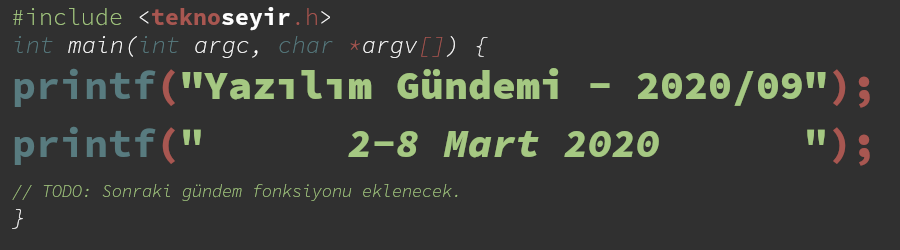
\includegraphics[width=.9\linewidth]{gorseller/yazilim-gundemi-banner.png}
\end{center}

\begin{center}
\href{../08/yazilim-gundemi-2020-08.pdf}{< Önceki Gündem} | \textbf{2-8 Mart 2020} | \href{../10/yazilim-gundemi-2020-10.pdf}{Sonraki Gündem >}

\href{https://teknoseyir.com/blog/yazilim-gundemi-2020-09}{TeknoSeyir'de Oku}
\end{center}

\section{Korona virüs yazılım şirketlerini \href{https://www.theverge.com/2020/3/5/21166686/coronavirus-amazon-google-facebook-microsoft-twitter-seattle-staff-remote-work}{uzaktan çalışmaya zorluyor}}
\label{sec:org06eec97}
Uzun bir zamandır tüm dünyanın gündemi, gün geçtikçe daha da fazla ülkede
görülmeye başlayan "Korona" virüsü. Elbette teknoloji ve dolayısıyla yazılım
sektörü de bu gündemden payını aldı. Amerika Birleşik Devletlerinde de vaka
sayılarının artmasıyla birlikte Microsoft, Facebook, Twitter ve Google gibi
büyük firmalar çalışanlarına "ofise gelmeyin uzaktan çalışabilirsiniz" demeye
başladı. Aynı zamanda sektörümüzle ilgili konferansların da çoğu ya iptal
edildi ya da çok ileri bir tarihe ertelendi.

Her ne kadar kötü bir olay nedeniyle de olsa firmaların artık uzaktan
çalışmaya sıcak bakması bence iyi bir gelişme. Ülkemizde pek fazla yaygın
olmasa da dünyada pek çok şirket uzaktan çalışma imkanını sunuyor zaten ama bu
olaylarla birlikte sayıları geçici olarak artsa bile faydasını gören
şirketlerin uzun dönem için de uzaktan çalışma imkanlarını
değerlendireceklerini düşünüyorum. Sadece şirket ve çalışanlar için değil,
şehir için de faydaları söz konusu olabilir. Nitekim Amazon ve Microsoft,
Seattle'daki ofisleri kapatmalarından dolayı Seattle şehrinin \href{https://www.geekwire.com/2020/seattle-morning-traffic-disappears-amazon-microsoft-others-enforce-remote-work-policies/}{trafiğinde gözle
görülür azalmalar olmuş}. Aynı şekilde konferans ve etkinliklerin de uzaktan
yapılacak olması, şirketlere ve organizasyonlara farklı bakış açıları
kazandıracaktır.
\section{Apple, App Store uygulama değerlendirme \href{https://www.developer-tech.com/news/2020/mar/05/apple-ios-developers-send-ads-push-notifications/}{rehberini güncelledi}}
\label{sec:org48751f0}
\href{https://www.developer-tech.com/}{DeveloperTech} sitesinin bu hafta yayınlandığı habere göre Apple, kendi
uygulama mağazası olan App Store'a uygulama gönderirken dikkat edilmesi
gerekenleri anlattığı dokümanı güncelledi.

Bu güncelleme ile birlikte artık geliştiriciler, bildirimleri kullanarak
kullanıcılara reklam içerikli mesajlar gönderebilecekler. Elbette
geliştiricilerin öncelikle bunun için kullanıcıdan izin almaları ve
kullanıcıya bu özelliği kapatma imkanının sunulması da gerekiyor.

Bir diğer önemli değişiklik ise üçüncü parti uygulamalar ve kullanıcı girişi
işlemlerini etkiliyor. Eğer uygulamanızda "Google ile giriş yap", "Facebook
ile giriş yap" gibi özellikleri sunuyorsanız, artık onların yanına \href{https://developer.apple.com/app-store/review/guidelines/\#sign-in-with-apple}{bir tane
daha eklemeniz gerekiyor}: "Apple ile giriş yap". Bu özelliği Apple geçtiğimiz
aylardaki bir etkinliğinde duyurmuştu ve gizlilik odaklı bir giriş sistemi
olduğunu söylemişti. Elbette bazı uygulamalar için ayrıcalık tanınmış durumda.
Uygulamanız bu listedeki maddeler ile uyumluysa, bu özelliği eklemek zorunda
değilsiniz:

\begin{itemize}
\item Eğer uygulamanız sadece kendi şirketinizin kullanıcı girişi sistemini kullanıyorsa,
\item Eğer uygulamanız kullanıcıların var olan eğitim ya da kurumsal hesaplarıyla
giriş yapabileceği eğitim için geliştirilmiş ya da kurumsal bir uygulama
ise,
\item Eğer uygulamanız bir devletin vatandaş tanımlama sistemlerini (e-devlet
gibi) kullanıyorsa,
\item Eğer uygulamanız sadece ilgili servisi kullanmaya yarayan bir istemci ise,
\end{itemize}

"Apple ile giriş yap" butonu eklemenize gerek yok. Bazı maddeleri iyi
çevirememiş olabilirim, bu nedenle en iyisi bir yanlış anlaşılmaya mahal
vermemek adına \href{https://developer.apple.com/app-store/review/guidelines/\#sign-in-with-apple}{dokümanın ilgili kısmına bir göz atın} :).
\section{Laravel 7 \href{https://laravel-news.com/laravel7}{sürümü yayınlandı}}
\label{sec:org8d6a0c0}
PHP ile web uygulamaları geliştirmeye yarayan popüler framework sistemlerinden
olan Laravel'in bu hafta içerisinde 7 numaralı yeni büyük güncellemesi
yayınlandı. 3 Mart günü duyurulan bu sürüm, 3 Eylül 2020'ye kadar hata giderme
güncellemesi, 3 Mart 2021'e kadar ise güvenlik güncelleştirmeleri almaya devam
edecek. Bu sürümle birlikte gelen bazı özellikler ise şu şekilde:

\subsection{Laravel Airlock}
\label{sec:orgf50a1ac}
Laravel'in içerisinde birçok konuda geliştiriciye kolaylıklar sağlayan alt
kütüphaneler mevcut. Artık bunlara bir yenisi daha ekleniyor: Laravel
Airlock. Kullanıcı girişi ve yetkilendirilmesi işlerini kolaylaştırıyor.
Elbette bu versiyondan önce de Laravel bu konuda kolaylıkları olan bir
framework idi fakat artık bu sistemin kendi bir adı var ve bazı ek özellikler
de gelmiş. Örneğin artık bir kullanıcıya birden çok erişim anahtarı (TOKEN)
tanımlayabilir ve bu erişim anahtarlarının kapsamını ve yapabileceklerini
sınırlayabiliyoruz.
\subsection{HTTP istemcisi}
\label{sec:orgcadc2b7}
Laravel, bu sürümle birlikte popüler PHP HTTP istemcilerinden biri olan
\href{https://github.com/guzzle/guzzle}{Guzzle} kütüphanesinin bazı parçalarını kendi içerisine ekledi. Artık web
uygulamamız içerisinden başka uygulamalar ya da siteler ile etkileşime
girerken daha zengin bir API'ye sahibiz. Örneğin bu şekilde bir POST isteği
yapıp, cevabını da kolayla kullanıcıya gösterebiliriz.
\begin{minted}[breaklines=true,breakanywhere=true,frame=lines, linenos, label=PHP, startinline]{php}
use Illuminate\Support\Facades\Http;

$response = Http::withHeaders([
    'X-First' => 'bir',
    'X-Second' => 'iki'
])->post('http://test.com/users', [
    'name' => 'Eren',
]);

return $response['id'];
\end{minted}

Bu sürümle birlikte gelen tüm özellik ve değişiklikler için \href{https://laravel.com/docs/7.x/releases}{bu sayfayı} ziyaret
edebilirsiniz. Ayrıca Laravel 6'dan Laravel 7'ye geçmek için de \href{https://laravel.com/docs/7.x/upgrade}{bu güncelleme
rehberi}nden faydalanabilirsiniz.
\section{PowerShell 7.0 \href{https://devblogs.microsoft.com/powershell/announcing-PowerShell-7-0/}{sürümü yayınlandı}}
\label{sec:org38de0e5}
Microsoft'un geçtiğimiz senelerde platformlar-arası (cross-platform)
çalışabilir hale getirdiği PowerShell, bu hafta içerisinde yeni sürümü
yayınladı.

Bu sürüm ile birlikte diğer shell'lerde olan bazı yeni operatörler
PowerShell'e de geldi. Örneğin artık pipeline operatörleri ile uygulamaları
ardı arına çalıştırabilir (\texttt{\&\&}) ya da birinin çıktısını diğerine
yönlendirebilirsiniz (\texttt{||}). Ben GNU/Linux dağıtımı kullandığım için bash
üzerinden bir örnek vereceğim ama uygulamaların windows karşılıklarıyla
aynısını PowerShell 7 üzerinde siz de çalıştabilirsiniz.
\begin{minted}[breaklines=true,breakanywhere=true]{shell}
wget http://ftp.linux.org.tr/linuxmint/iso/stable/19.3/linuxmint-19.3-cinnamon-64bit.iso && shutdown -h now
\end{minted}
Yukarıdeki gibi bir komutu çalıştırarak önce ilgili dosyayı indirebilir,
ardından ise sisteminizi kapatabilirsiniz.

Yeni sürümle ilgili detaylı bilgiler ve güncelleme rehberi için konu başlığına
eklediğim bağlantıya tıklayabilirsiniz.
\section{Yaklaşan Etkinlikler}
\label{sec:org2a4ce60}
\begin{longtable}{|p{8cm}|l|l|}
\hline
Etkinlik İsmi & Yeri & Tarihi\\
\hline
\endfirsthead
\multicolumn{3}{l}{Önceki sayfadan devam ediyor} \\
\hline

Etkinlik İsmi & Yeri & Tarihi \\

\hline
\endhead
\hline\multicolumn{3}{r}{Devamı sonraki sayfada} \\
\endfoot
\endlastfoot
\hline
\href{https://www.meetup.com/Open-Source-Analytics-Istanbul/events/269198806/}{Deploy AI - Community Day} & Online & 10 Mart 15:00\\
\href{https://kommunity.com/ngturkey/events/webinar-angular-9-ivy-scully-ve-test-harness-angular-turkey}{Angular 9, Ivy, Scully ve Test Harness - Angular Turkey} & Online & 11 Mart 19:30\\
\href{https://www.meetup.com/bilisimtoplulugu/events/269127026/}{C\# Günleri} & İstanbul & 12 Mart 11:00\\
\href{https://www.meetup.com/istanbul-yapay-zeka-toplulugu/events/269128397/}{AI?!: Yapay Zekâda Pratik ve Teori} & İstanbul & 12 Mart 15:00\\
\href{https://www.meetup.com/laravelistanbul/events/269059351/}{TDD API Development, the right way} & İstanbul & 12 Mart 19:00\\
\href{https://kommunity.com/btorgtr/events/devops-workshop-bilisim-kahvesi-lab}{DevOps Workshop, Bilişim Kahvesi Lab} & İstanbul & 12 Mart 19:30\\
\href{https://www.meetup.com/Coffee-And-React-Native-\%25C4\%25B0stanbul/events/hhtdprybcfbsb/}{Coffee and React Native} & İstanbul & 14 Mart 11:00\\
\href{https://www.meetup.com/IzmirGophers/events/269152779/}{HTML5 Canvas API ile 2D, Graph ve WebGL Uygulamalari ve Go ile HTTP2MQTT} & İzmir & 15 Mart 15:00\\
\href{https://www.meetup.com/bilisimtoplulugu/events/269153853/}{Yapay Zeka ve Çalışma Alanları} & İstanbul & 16 Mart 13:30\\
\href{https://kommunity.com/turkey-openstack-meetup/events/openinfra-day-turkey}{OpenInfra Day Turkey 2020} & İstanbul & 17 Mart 09:00\\
\href{https://www.meetup.com/Turkiye-Yapay-Zeka-\%25C4\%25B0nisiyatifi/events/xztxmrybcfbxb/}{TRAI Meet-Up - no.32 İleri Algoritmalar} & İstanbul & 18 Mart 18:00\\
\href{https://kommunity.com/devops-turkiye/events/docker-7-yas-partisi}{Docker 7. Yaş Partisi!} & İstanbul & 18 Mart 18:45\\
\href{https://kommunity.com/software-craftsmanship-turkey/events/scturkey-meetup}{Kendimize İlham Olabilmek (Software Craftsmanship Turkey)} & İstanbul & 18 Mart 19:00\\
\href{https://kommunity.com/cloud-and-serverless-turkey/events/azure-functions-on-kubernetes-istanbul}{Azure Functions on Kubernetes} & İstanbul & 19 Mart 18:30\\
\href{https://www.meetup.com/Istanbul-Hackers/events/268972005/}{İstanbul Coders Reunion} & İstanbul & 19 Mart 19:00\\
\href{https://kommunity.com/setur/events/bir-fincan-dolusu-ufuk-acan-sohbetler-coffee-talks}{Bir fincan dolusu, ufuk açan sohbetler: Coffee Talks} & İstanbul & 20 Mart 10:30\\
\href{https://www.meetup.com/GDGAnkara/events/268276284/}{Women Techmakers Ankara IWD'20} & Ankara & 21 Mart 09:00\\
\href{https://www.meetup.com/ING-\%25C4\%25B0novasyon-Merkezi/events/269254711/}{Python Öğren - Python'a 4 Saatte Başlangıç} & İstanbul & 22 Mart 10:00\\
\href{https://www.meetup.com/ING-\%25C4\%25B0novasyon-Merkezi/events/269254823/}{LearnDocker İstanbul: Docker'a Giriş} & İstanbul & 22 Mart 15:00\\
\hline
\end{longtable}
\section{Diğer Haberler}
\label{sec:org073052c}
\begin{itemize}
\item Yazılımcılar için sosyal medya özelliği olan Dev.to, 8 Mart Dünya Emekçi
Kadınlar günü için kadınların programlamaya başlama \href{https://dev.to/t/shecoded}{hikayelerini
anlatabileceği özel bir sayfa hazırladı}.
\item Google, Korona virüsü nedeniyle iptal edilen organizasyonların ve okulların
kullanabilmesi için \href{https://gsuite.google.com/products/meet/}{Hangout Meet} hizmetine \href{https://cloud.google.com/blog/products/g-suite/helping-businesses-and-schools-stay-connected-in-response-to-coronavirus}{sınırlı süre için ücretsiz paket
ekledi}.
\item Korona virüsü nedeniyle iptal edilen organizasyonlar:
\begin{itemize}
\item Google I/O konferası \href{https://techcrunch.com/2020/03/03/google-cancels-its-2020-i-o-developer-conference/}{online olarak düzenlenecek}.
\item Atlassian Summit 2020 \href{https://www.atlassian.com/company/events/summit}{etkinliği iptal edildi}.
\item KubeCon etkinliği 17 - 20 Kasım 2020 \href{https://events.linuxfoundation.org/kubecon-cloudnativecon-europe/attend/novel-coronavirus-update/}{tarihine ertelendi}.
\end{itemize}
\item NodeJS v13.10.0 \href{https://nodejs.org/en/blog/release/v13.10.0/}{sürümü yayınlandı}.
\item VueJS kütüphanesinin v3.0.0-alpha \href{https://github.com/vuejs/vue-next/releases/tag/v3.0.0-alpha.8}{sürümü yayınlandı}.
\item Angular Framework 9.0.5 \href{https://github.com/angular/angular/releases/tag/9.0.5}{sürümü yayınlandı}.
\item Kotlin programlama dilinin 1.3.70 \href{https://blog.jetbrains.com/kotlin/2020/03/kotlin-1-3-70-released/}{sürümü yayınlandı}.
\item Rollup bundler aracının 2.0.0 \href{https://github.com/rollup/rollup/releases/tag/v2.0.0}{sürümü yayınlandı}.
\item HTTP istek ve cevaplarını OpenAPI standartlarına göre denetleyen openapi-cop
aracının \href{https://github.com/EXXETA/openapi-cop}{ilk stabil versiyonu 1.0.0 yayınlandı}.
\end{itemize}
\section{Lisans}
\label{sec:org32cebbd}
\begin{center}
\begin{center}

\includegraphics[height=1.5cm]{../../../img/CC_BY-NC-SA_4.0.png}
\end{center}

\href{yazilim-gundemi-2020-09.pdf}{Yazılım Gündemi - 2020/09} yazısı \href{https://erenhatirnaz.github.io}{Eren Hatırnaz} tarafından \href{http://creativecommons.org/licenses/by-nc-sa/4.0/}{Creative Commons
Atıf-GayriTicari-AynıLisanslaPaylaş 4.0 Uluslararası Lisansı} (CC BY-NC-SA 4.0)
ile lisanslanmıştır.
\end{center}
\end{document}
